\Chapter{Mérések, összehasonlítások}

Ebben a fejezetben megvizsgáljuk a program különböző részeit futás idő szempontjából. Ezek több csoportba bonthatjuk. Egyes részek futási ideje nagyban függ a kezelt adatok mennyiségétől, más részeket pedig elegendő lehet egyszer elvégezni. Illetve vannak azok a részek, amelyik nem csak az adatmennyiségtől függnek, hanem magától az algoritmustól vagy a párhuzamosítás mértékétől is.

\Section{Állandó idejű részek}
Ennek a résznek a vizsgálata a legegyszerűbb, mégis ugyan olyan fontos hiszen, hogy a program valóban hatékony legyen ezeket az időket is vissza kell nyerni a lekérdezéseknél.

Kernelkód beolvasása a fájlból.
40 mikroszekundum.

Kapcsolat létrehozása az adatbázis szerverrel:
16500 mikroszekundum.

OpenCL: driver kontextus, parancssor
50 000 mikroszekundum

Program létrehozása és felépítése az eszközhöz
1000 mikroszekundum

\Section{Adatmennyiségtől függő részek}

A hatékonyság mérésének bonyolultabbik része következik. Itt vizsgáljuk meg, hogyan érdemes mozgatni az adatokat a számítógépen belül úgy, hogy nyereséges maradjon a kód.

\SubSection{A MySQL lekérdezés sebessége}
Ezt a sebességet legpontosabban úgy kaphatjuk meg ha a program következő két sorának idejét vizsgáljuk.
\begin{python}
pstmt = con->prepareStatement(command);
res = pstmt->executeQuery();
\end{python}
Ahhol \texttt{command} egy \texttt{String} az SQL parancs és a következő módon áll össze:
\begin{python}
range=32768;
    while(i <= 1048576){
    		command = "SELECT * FROM speedtest_1048576 Limit " 
    			+ to_string(i);
    		. . .
   	 	i+=range;
    }
\end{python}
Ezen kívül a grafikonon látható tüskék mértékének csökkentése érdekében minden lekérdezést 5x futtattam és idejüket átlagoltam.
\begin{itemize}
\item A LIMIT hozzáadása a lekérdezéshez nem növeli annak idejét.
\item A tábla tartalmaz elsődleges kulcsot, enélkül a lekérdezések ideje nő.
\item A lekérdendő oszlopokat manuálisan módosítottam a programban. 
\begin{itemize} 
\item \texttt{SELECT c1p1 FROM ...}
\item \texttt{SELECT c1p1, c2 FROM ...} 
\item \texttt{SELECT c1p1, c2, c3 FROM ...} 
\item \texttt{SELECT * FROM ...} 
\end{itemize}
\end{itemize}

\begin{figure}[h!]
\centering
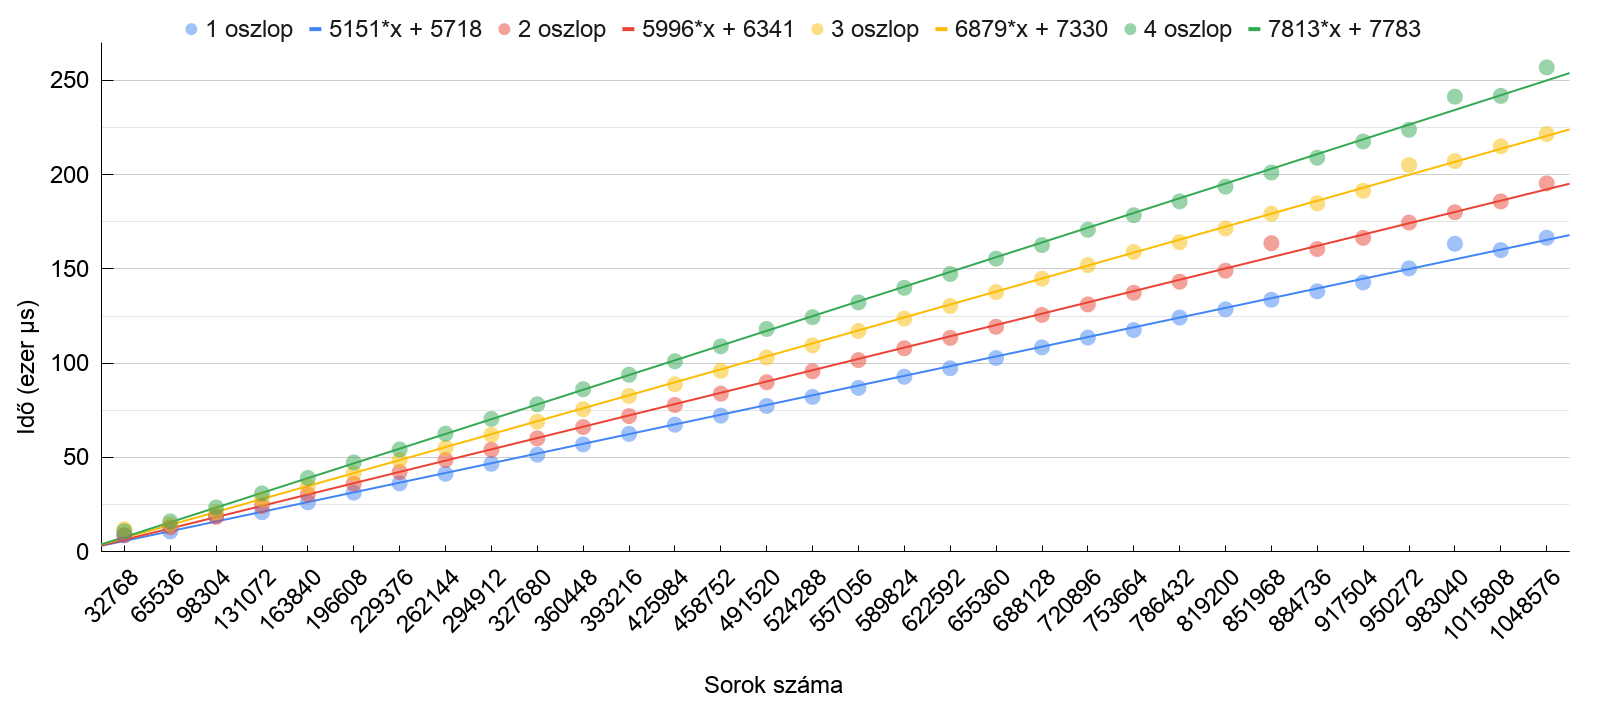
\includegraphics[width=\textwidth]{images/sqlquery.png}
\caption{Az SQL lekérdezési sebessége}
\label{fig:schema}
\end{figure}
%BETŰMÉRET NAGYÍTÁSRA SZORUL
Az ábrán, egyértelműen látható, hogy a sorok számának növekedésével az idő is lineárisan nő.
Jelmagyarázatnál látható egyenes egyenletekből becsléseket lehet készíteni adott sorszámhoz. Tegyük fel, hogy a négy oszlop felett az időnövekedés lineáris, így több oszlopra egyszerű szorzással megkaphatjuk az időket.

4 és 6 oszlop esetén:
$$ x = \text{sorok száma}/32768 - 1 $$
$$ 7813 * \text{sorok száma} + 7783 = \text{lekérdezés ideje}$$
$$ \text{lekérdezés ideje} * 1.5 = \text{lekérdezés ideje 6 oszlopra} $$


\SubSection{A query válaszának átmásolása a struktúra tömbbe}
Az előző alfejezetben kapott választ át kell másolni saját típusú tömbbe, hogy megfelelően tudjuk kezelni. Ez egy rendkívül időigényes rész. 

A mért program szakasz:
\begin{python}
int i = 0;
*T1_size = res->rowsCount();
*T1 = (Table1Type*) malloc(sizeof(Table1Type) * *T1_size);

while (res->next())
	{
		T1[0][i].c1p1 = res->getInt("c1p1");
		T1[0][i].c2 = res->getInt("c2");
		T1[0][i].c3 = res->getInt("c3");
		T1[0][i].c4 = res->getInt("c4");
		i++;
	}
delete res;
delete pstmt;
\end{python}

Itt a válaszból lekérdezzük a méretet, majd ez alapján létrehozzuk a saját objektumunkat a memóriában, ezután egyesével belemásoljuk 
a kapott adatokat soronként.
Az mérési módszer megegyezik az előzőekben használtakkal.
A texttt{res} és texttt{pstmt} törlése időméréskor nagyon fontos, ugyanis ennek kihagyása miatt a memória megtelhet!


\begin{figure}[h!]
\centering
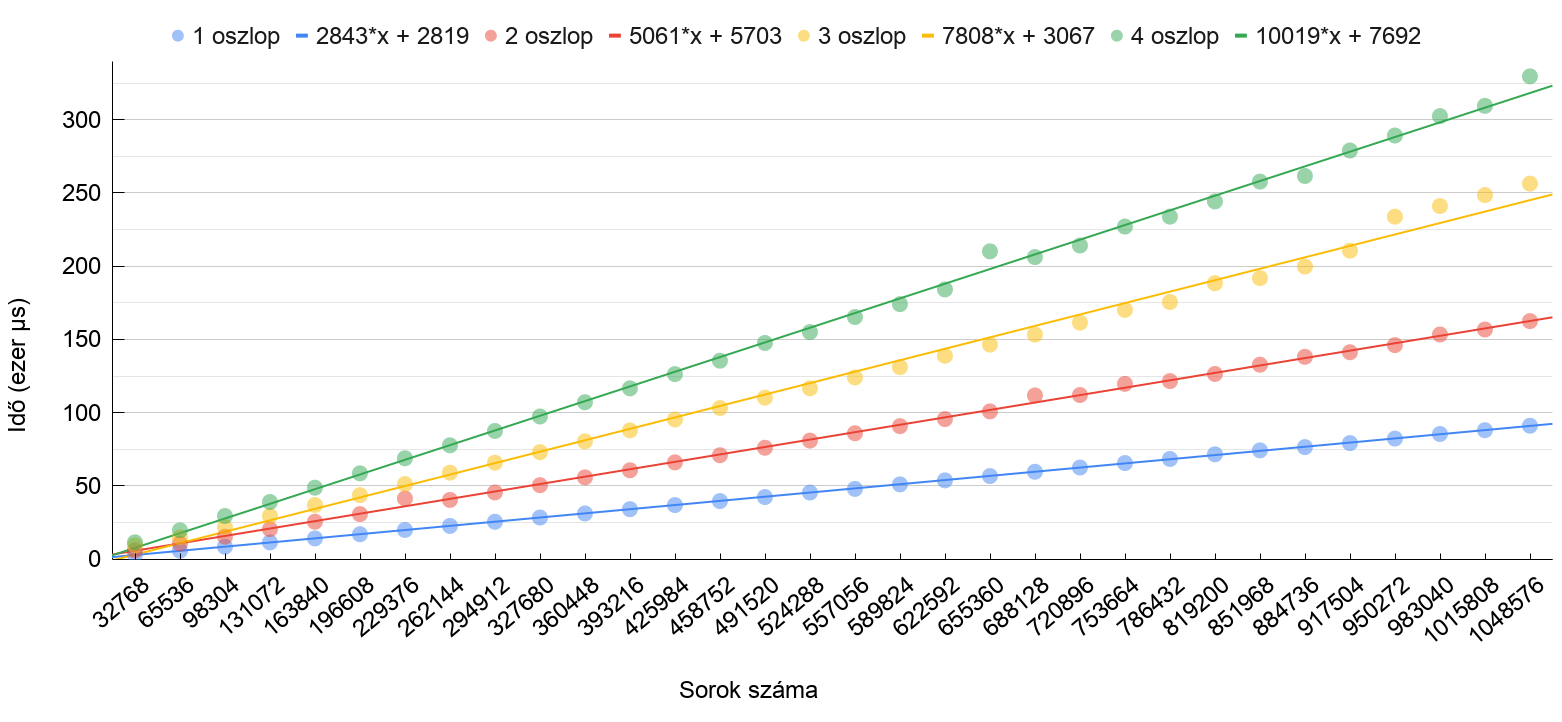
\includegraphics[width=\textwidth]{images/ccopy.png}
\caption{Adatok másolása saját tömbbe}
\label{fig:schema}
\end{figure}

A grafikonon két dolgot vehetünk észre azonnal. Az egyik az, hogy ez a folyamat lassabb mint maga a lekérdezés a másik pedig, hogy drasztikusabb a növekedés az oszlopok számának sokasodásával.
Tegyük fel, hogy 4 oszlop felett már nincs szignifikáns eltérés az időnövekedésben. Ekkor használhatjuk az előbb is használt módszert a becslésekhez.

Másolás becslése 4 és 6 oszlop esetén:
$$ x = \text{sorok száma}/32768 - 1 $$
$$ 10019 * x + 7692 = \text{másolás ideje}$$
$$ \text{másolás ideje} * 1.5 = \text{másolás ideje 6 oszlopra} $$

\SubSection{Adatok bemásolása a pufferekbe}

Az adatok átmásolása az OpenCL puffereibe szintén egy olyan része a programnak, ami sok időt emészthet fel.
Vizsgált rész:

\begin{python}
int range=65536;
while( range <= 1048576){
 clStatus = clEnqueueWriteBuffer(command_queue, Table1_clmem,
  CL_TRUE, 0, range * sizeof(Table1Type), t1, 0, NULL, NULL);
 clStatus = clEnqueueWriteBuffer(command_queue, Table_size_clmem,
  CL_TRUE, 0, sizeof(int), &t1_size, 0, NULL, NULL);
 clStatus = clEnqueueWriteBuffer(command_queue, Interval_size_clmem,
  CL_TRUE, 0, sizeof(int), &interval_size, 0, NULL, NULL);
 clStatus = clFinish(command_queue);
	range += 65536;
}
\end{python}

A mérés a belső 4 sorra vonatkozik. 

\begin{figure}[h!]
\centering
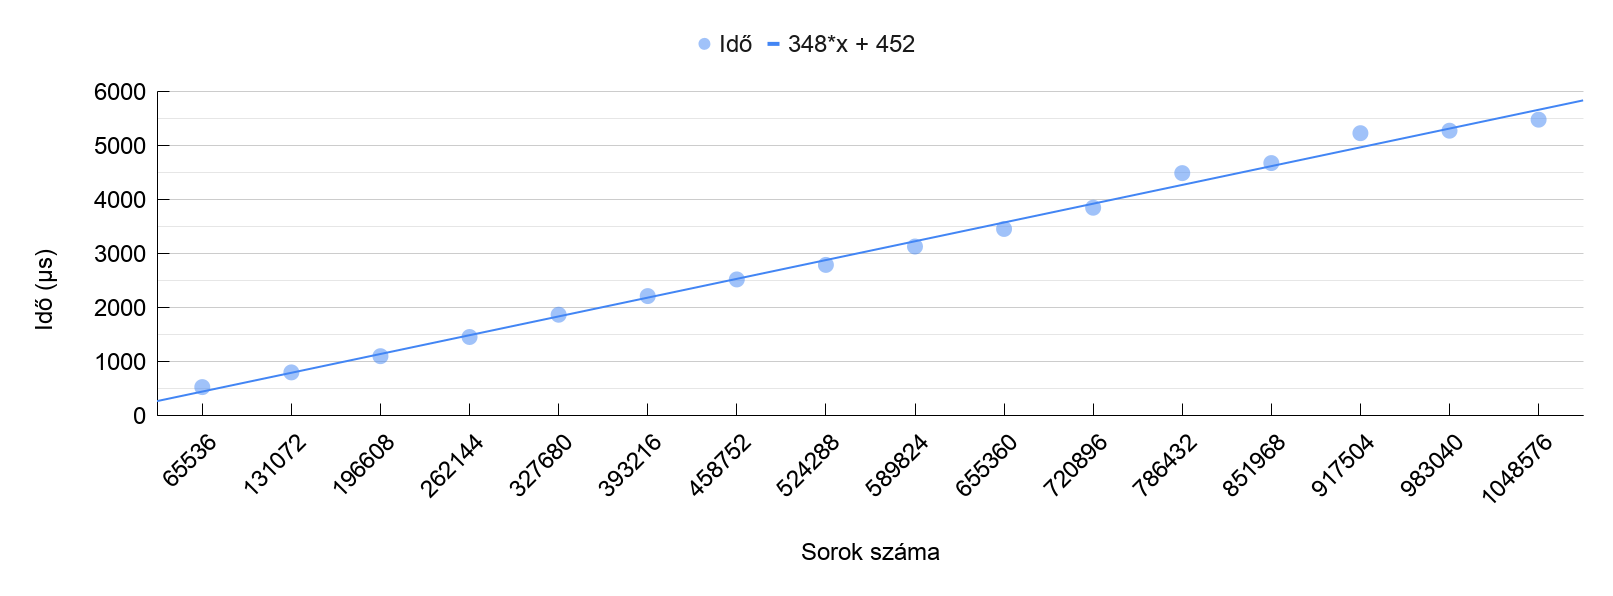
\includegraphics[width=\textwidth]{images/inpuffer.png}
\caption{Adatok kimásolása 2.}
\label{fig:schema}
\end{figure}

Mivel ebben az esetben a másolás egybefüggő memória területre vonatkozik, nem pedig elemenkénti hivatkozás, ezért elegendő egyetlen mérés.
A grafikonon egy 4 oszlopos tábla átmásolásának a sebessége látható. Ebből Több vagy kevesebb oszlopra a becslés egyszerű szorzásokkal megkapható.

4 és 3 oszlop esetén:
$$ x = \text{sorok száma} / 65536 $$
$$ 348*x + 452 = \text{pufferbe másolás ideje} $$ 
$$ \text{pufferbe másolás ideje} * 0.75 = \text{3 oszlopos pufferbe másolás ideje}  $$



\SubSection{Adatok kimásolása a pufferekből}

A program ezen részének hatékonysága már egy komplexebb vizsgálatot igényel.
Nézzük az első kiolvasási módszert, amikor a teljes válasz listát illetve a hozzá tartozó számlálót másoljuk ki.
Jelen mérésnél a lista csak egyetlen indexet tartalmaz. 

\begin{figure}[h!]
\centering
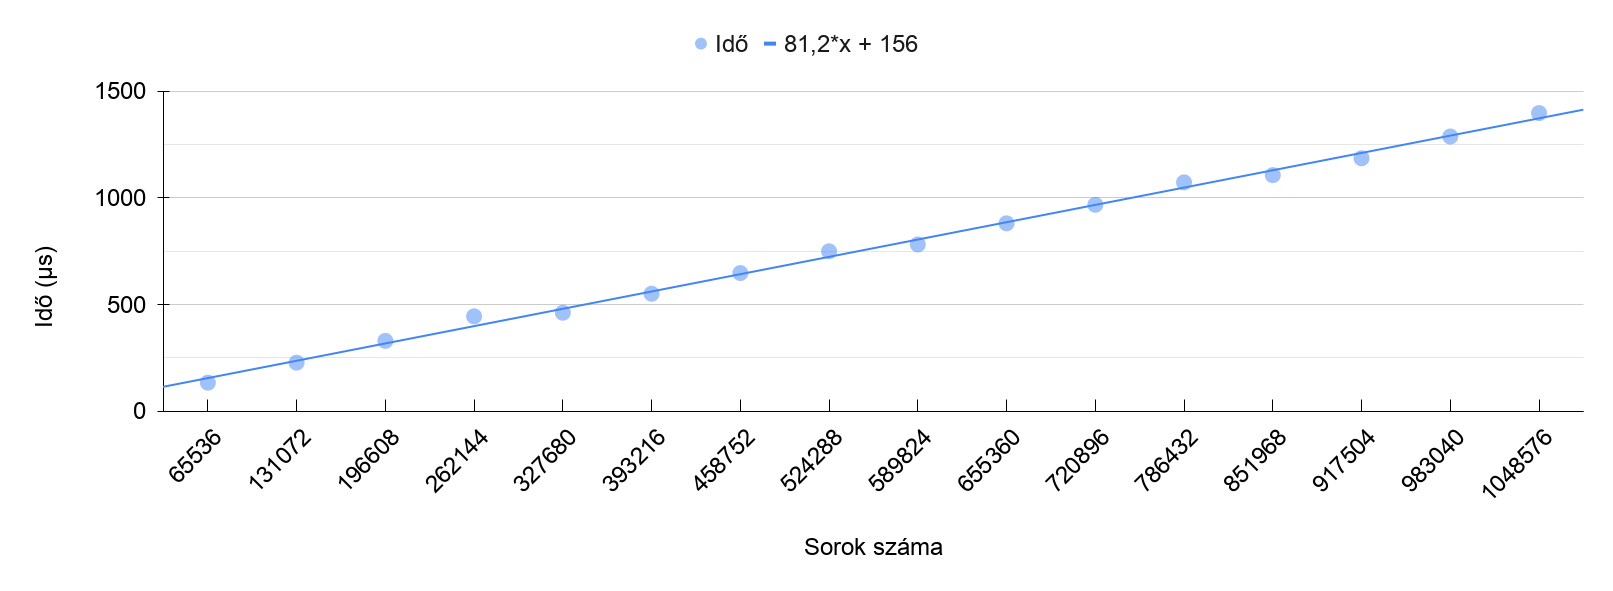
\includegraphics[width=\textwidth]{images/outpuffer.png}
\caption{Adatok kimásolása 2.}
\label{fig:schema}
\end{figure}

$$ 81,2*x + 156 = \text{puffer kiolvasási ideje} $$ 
Az előzőhöz hasonlóan itt is egy memória darabot másolunk, ennek szorzásával megkapjuk mennyi időbe telne a kiolvasás indexpárok vagy számított értékek hozzáadása esetén.
Ne felejtsük el, hogy ehhez tartozik egy számláló, ami jelen esetben a képlethez képest az elemszám gyöke, de két érték esetén már csak a felének a gyöke.
Ez azt jelenti, hogy $2^{20}$ -on érték esetén is a kiolvasási ideje csak megközelítőleg 37$\mu\text{s}$


A másik módszer miszerint nem olvassuk ki azonnal a választ, hanem alkalmazzuk az előző fejezetben taglalt optimalizálási eljárást.
Ennek hatékonysága a sok kisebb olvasás miatt függ az eredmények számától. Ennek méréséhez módosítani kell a kernel kódot, ezért maunálisan végeztem a méréseket, vagyis a szűrési feltételeket úgy módosítottam, hogy a találatok száma megfelelően változzon.
Fontos figyelembe venni, hogy a számok véletlenszerűek a táblázatban.

\begin{figure}[h!]
\centering
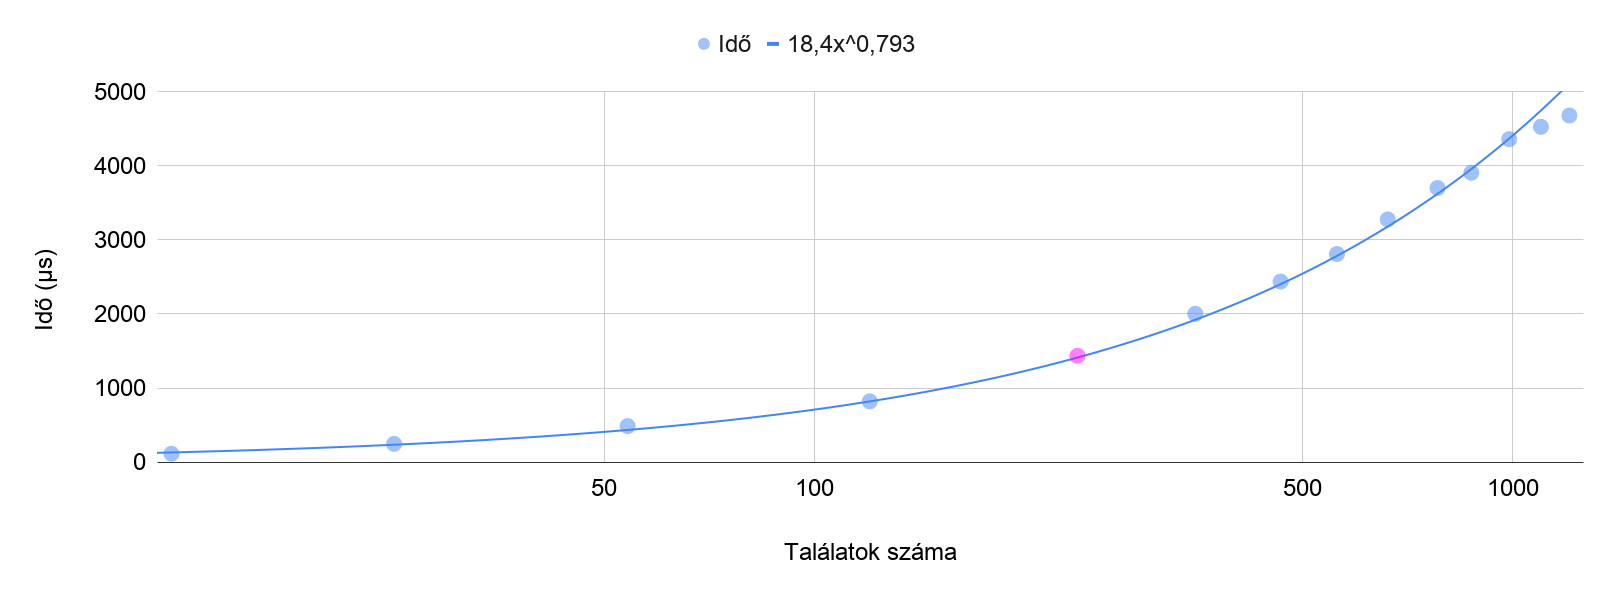
\includegraphics[width=\textwidth]{images/outpuffer2.png}
\caption{Adatok kimásolása 2.}
\label{fig:schema}
\end{figure}

Végeredményként látjuk, hogy ez a fajta kiolvasás rendkívül hatékony, de csak abban az esetben, ha a találatok száma minimális.
238 találatnál a módszer elérte azt az időt, ami alatt el lehet végezni a teljes másolást egy darabban.
\begin{figure}[h!]
\centering
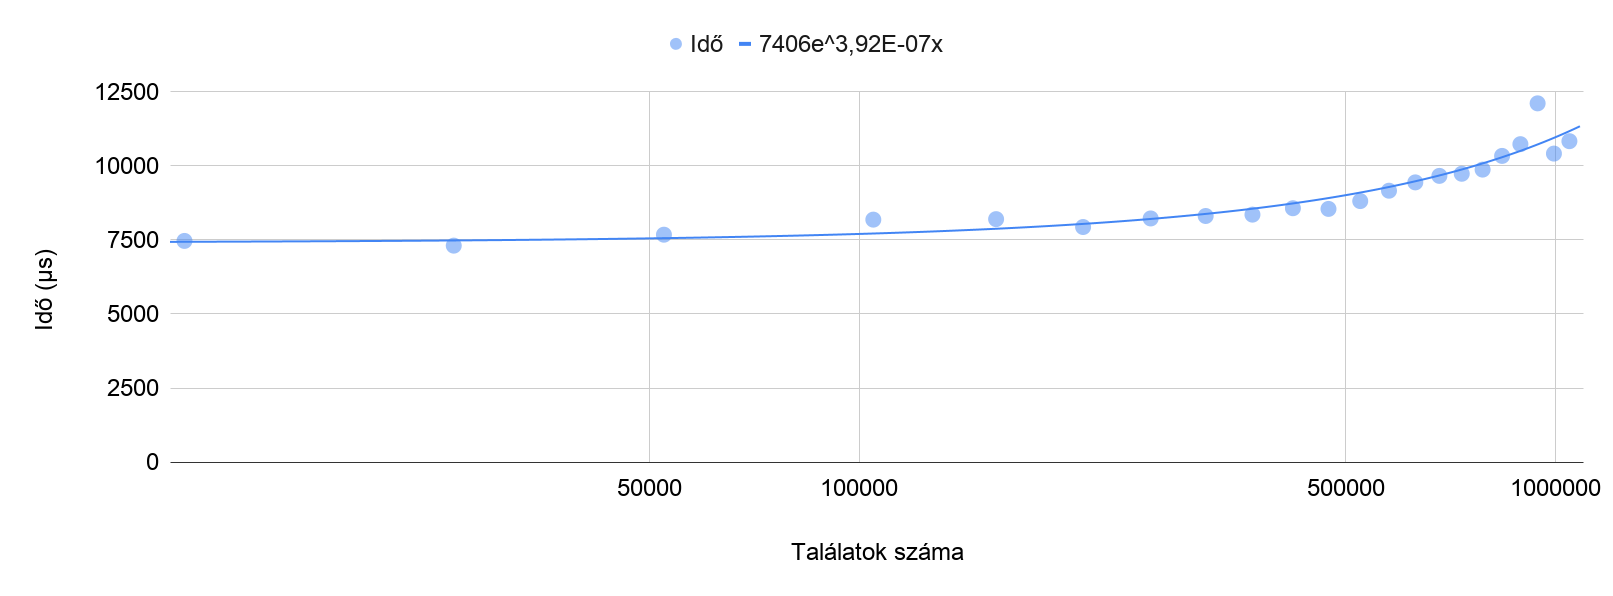
\includegraphics[width=\textwidth]{images/outpuffer3.png}
\caption{Adatok kimásolása 2.}
\label{fig:schema}
\end{figure}

\newpage
\SubSection{A globális méretből adódó sebességek}

A megfelelő globális méret meghatározása futási idő szempontjából nagyon fontos.

Túl nagy globális méret hatásai:
\begin{itemize}
\item A lokális méret korlátai miatt túl sok csoport jön létre, így azok feldolgozása soros lesz.
\item A kimeneti számláló mérete megnő, ennek kiolvasása több idő, és alacsony találati szám mellett a fölösleges ellenőrzések száma szignifikáns lehet.
\end{itemize}

Túl alacsony globális méret hatásai:
\begin{itemize}
\item A lokális méretet is szükséges lehet csökkenteni. Ha túl alacsony, akkor egyetlen munkaelem fogja végrehajtani, a párhuzamosság teljesen megszűnik.
\item A kimeneti számláló mérete alacsony, kevés visszatérő értéknél a kiolvasás gyors.
\end{itemize}


A méréseket ezen pontok alapján a következők szerint végeztem.

A globális méret változzon 1 - $2^{20}$ értékig, a lokális pedig 1 - 1024 ig négyzetes lépcsőkkel, az oszthatóságra figyelve.

A vizsgált kódrészlet:
\begin{python}  
timer.start();

clStatus = clEnqueueNDRangeKernel(command_queue, kernel, 1, NULL, 
	&global_size, &local_size, 0, NULL, NULL);

clStatus =
	clEnqueueReadBuffer(command_queue, Result_indexes_list_clmem, 
	CL_TRUE, 0, global_size* sizeof(int), 
	result_counter, 0, NULL, NULL);
	
clStatus = clEnqueueReadBuffer(command_queue, TableResult_clmem, 
	CL_TRUE, 0, t1_size * sizeof(TableResultType), 
	result  , 0,NULL, NULL);

clStatus = clFinish(command_queue);
clStatus = clFlush(command_queue);

for(int i=0; i<global_size; i++)
{
	for(int j = 0; j < result_counter[i]; j++ )
	{

	}
}
myfile << timer.elapsedMicroseconds() << "," ;  
\end{python}

Szembetűnő lehet az egymásba ágyazott két ciklus. Azért szerepel ez kódrészlet a mérésekbe, hogy az eredményeken való végiglépegetés idejének nagyságrendje valamilyen módon meghatározható legyen. Fontos megjegyezni, hogy a fordítás során nem kerül figyelmen kívül hagyásra ez a két ciklus.

A következő diagrammon látható részletesen mely program szakasz mennyi időbe telik.
Minden esetben a Lokális méret 32 és a visszatérő értékek száma körülbelül $50\%$. Az eredményben csak index szerepel.

\begin{figure}[h!]
\centering
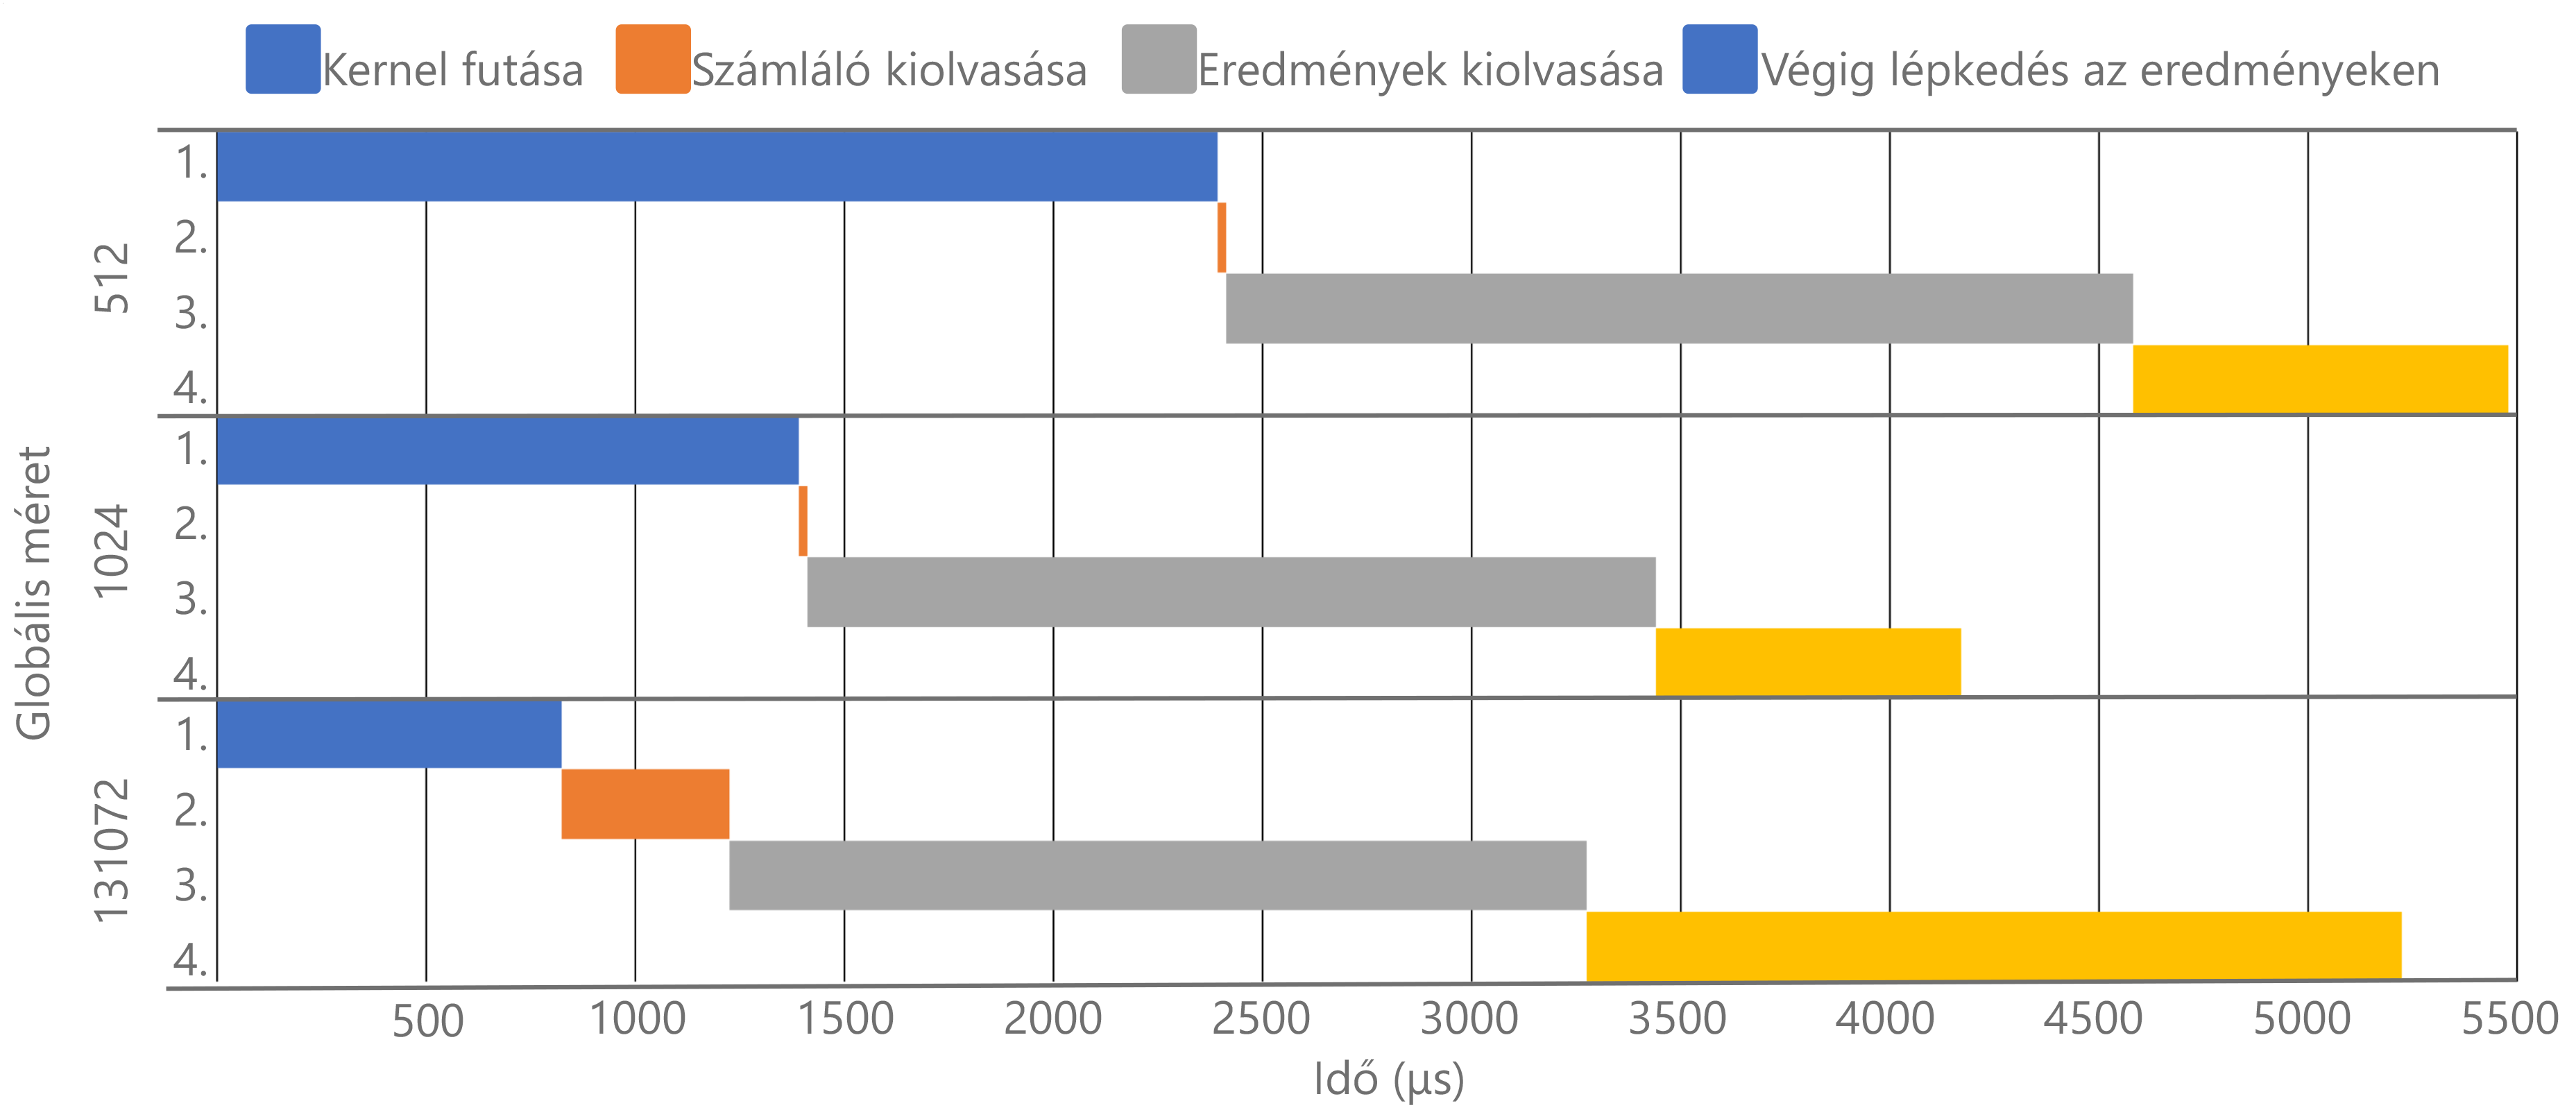
\includegraphics[width=\textwidth]{images/gantt.png}
\caption{Programszakaszok ideje.}
\label{fig:schema}
\end{figure}

Látható, hogy a túl alacsony globális méret túl magas kernel futási időt eredményez. Túl nagy méret esetében pedig az eredmények kezelésének ideje válik számításigényessé.

\newpage

Az eredményt megvizsgálva látható, hogy van egy optimális globális méret tartomány $262144$ és $1024$ között.
Azt is észrevehetjük, hogy bizonyos lokális méretek ebben a tartományban drasztikusan rosszabb eredményt mutatnak.
A 16 és 32 -es méretek állnak legközelebb az ideális futási időhöz.
\begin{figure}[h!]
\centering
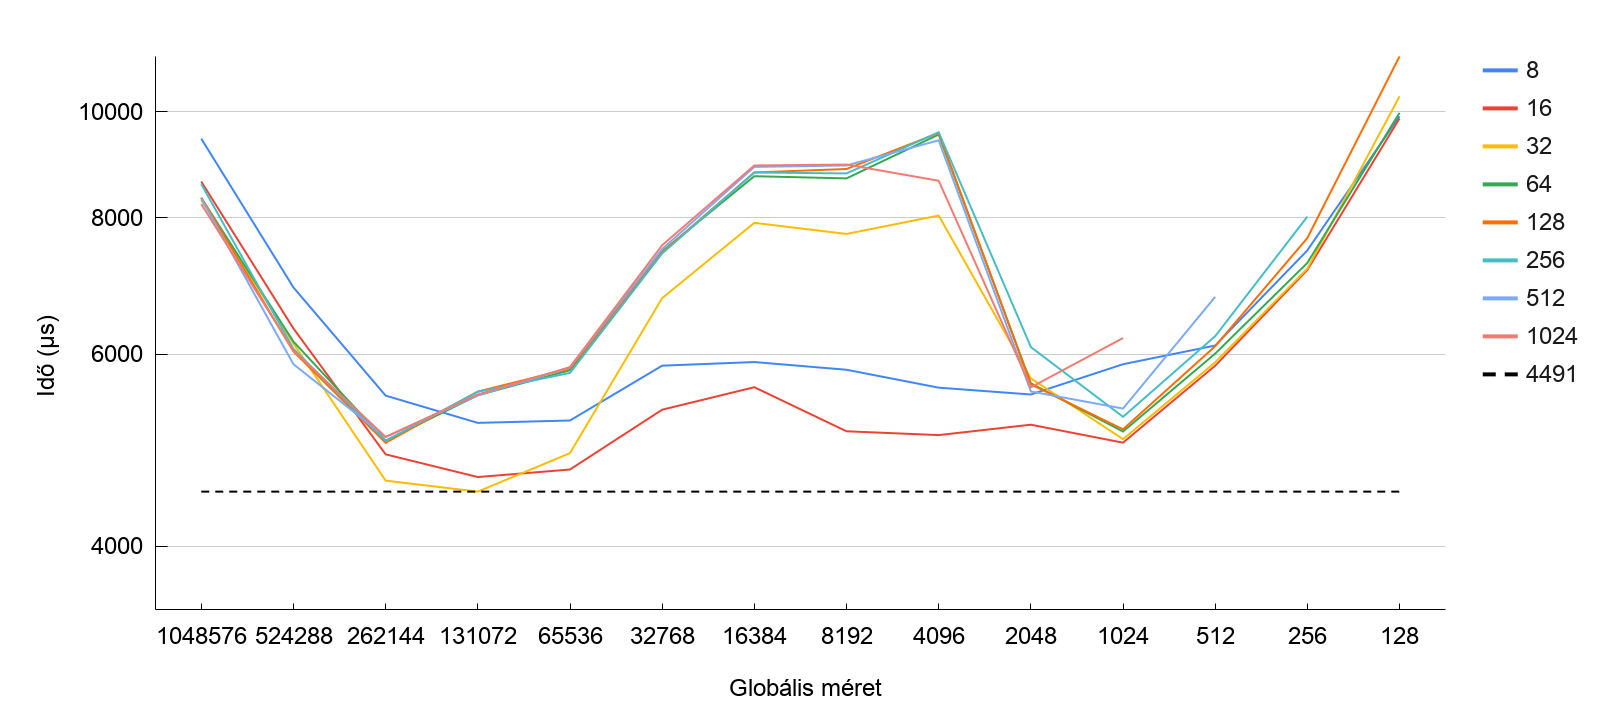
\includegraphics[width=\textwidth]{images/gs_1_max.png}
\caption{Maximális találat, az eredmény csak index.}
\label{fig:schema}
\end{figure}


A második grafikonon egy olyan mérés látható, ahol a kernelben található feltételt úgy állítottam be, hogy megközelítőleg csak a tábla méretének 10\% -ával térjen vissza a lekérdezés.
Azt láthatjuk, hogy az előző középen lévő hullám lesimul, ez részben annak köszönhető hogy a kernel futási ideje csökken azzal, hogy nem kell annyi indexet az eredmény tömbbe írnia.

\begin{figure}[h!]
\centering
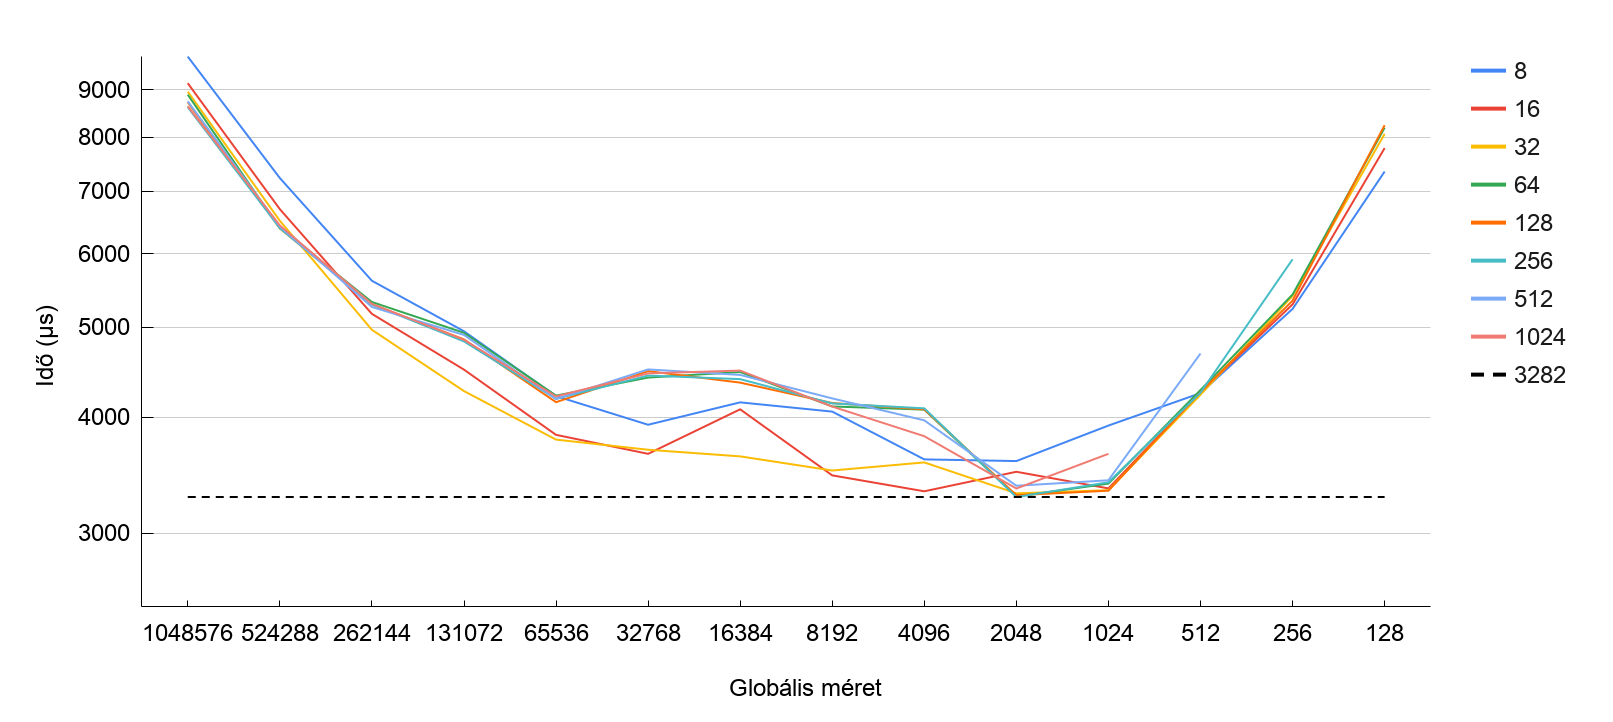
\includegraphics[width=\textwidth]{images/gs_1_10.png}
\caption{kb. 10\% találat, az eredmény csak index.}
\label{fig:schema}
\end{figure}

Azoknál a lekérdezéseknél, a kernelnek nem csak egy indexel kell visszatérnie hanem több kalkulált értékkel is, ott is hasonló grafikonokat kapunk. De a kernel növekvő munkája és a megnövekedett adatmennyiség kiolvasása miatt a középen lévő hullám nagyobb és nehezebben lapul le.

Ezek alapján meghatározható, hogy az 
\newpage
\Section{Hatékonyság a gyakorlatban}

A hatékonyság megállapításához a \texttt{A MySQL lekérdezés sebessége} részben használt módszert fogom alkalmazni.
Azt már most észrevehetjük, hogy ezen oknál fogva a szerverre való csatlakozás sebességét elhanyagolhatjuk ugyanis minden kliensnek szüksége van rá. 

\SubSection{Egy táblás lekérdezés}

\begin{python}
SELECT * FROM speedtest_1048576 WHERE c3 = 1 AND c4 > 5001
\end{python}

A Connector lekérdezési ideje: 178061 


Ezzel szemben az OpenCL megvalósítás.
\begin{python}
38      Read kernel file: Done.
17227   Server connection: Done.
264060  MySQL query: Done.
316775  Copy to the arrays: Done.
0       Define sizes: Done.
96585   Define queue: Done.
24      Create buffer: Done.
6298    Write to the buffer: Done.
21      Create the program: Done.
1260    Build the program: Done.
5       Createing kernel: Done
1       Setting kernel arguments: Done.
1917    Running the kernel: Done.
2191    Reading the result: Done.
\end{python}

Ha a programot buildelni kell az ideje 1260 helyett 71396.

Bontsuk két szakaszra a programot.
Felkészülés az adatfeldolgozásra. 
$$ 38 + 17227 + 316755 + 96585 + 24 + 6298 + 21 + 1260 + 6 = 438214 $$

Adatfeldolgozás és kimenetre küldés.

$$ 1917 + 2191 $$